% Asset ID: FA22FurtherCentreOfMassTikZ-002
% Source: Teacher transcript and slide PDF polar sector/arc examples
% Related lesson section: #9 Visual Asset Integration; #8.6 Optional Enrichment
% Purpose: Optional enrichment visual for sector and arc derivations using small angle d\theta.
\documentclass[tikz,border=8pt]{standalone}
\usepackage{amsmath}
\usepackage{xcolor}
\usetikzlibrary{arrows.meta,calc}
\definecolor{canvas}{HTML}{FAF9F6}\definecolor{ivory}{HTML}{FFFFF0}\definecolor{ink}{HTML}{2C2C2E}\definecolor{linegray}{HTML}{E5E5EA}\definecolor{gold}{HTML}{C5A059}\definecolor{softpink}{HTML}{FBEFEF}
\begin{document}
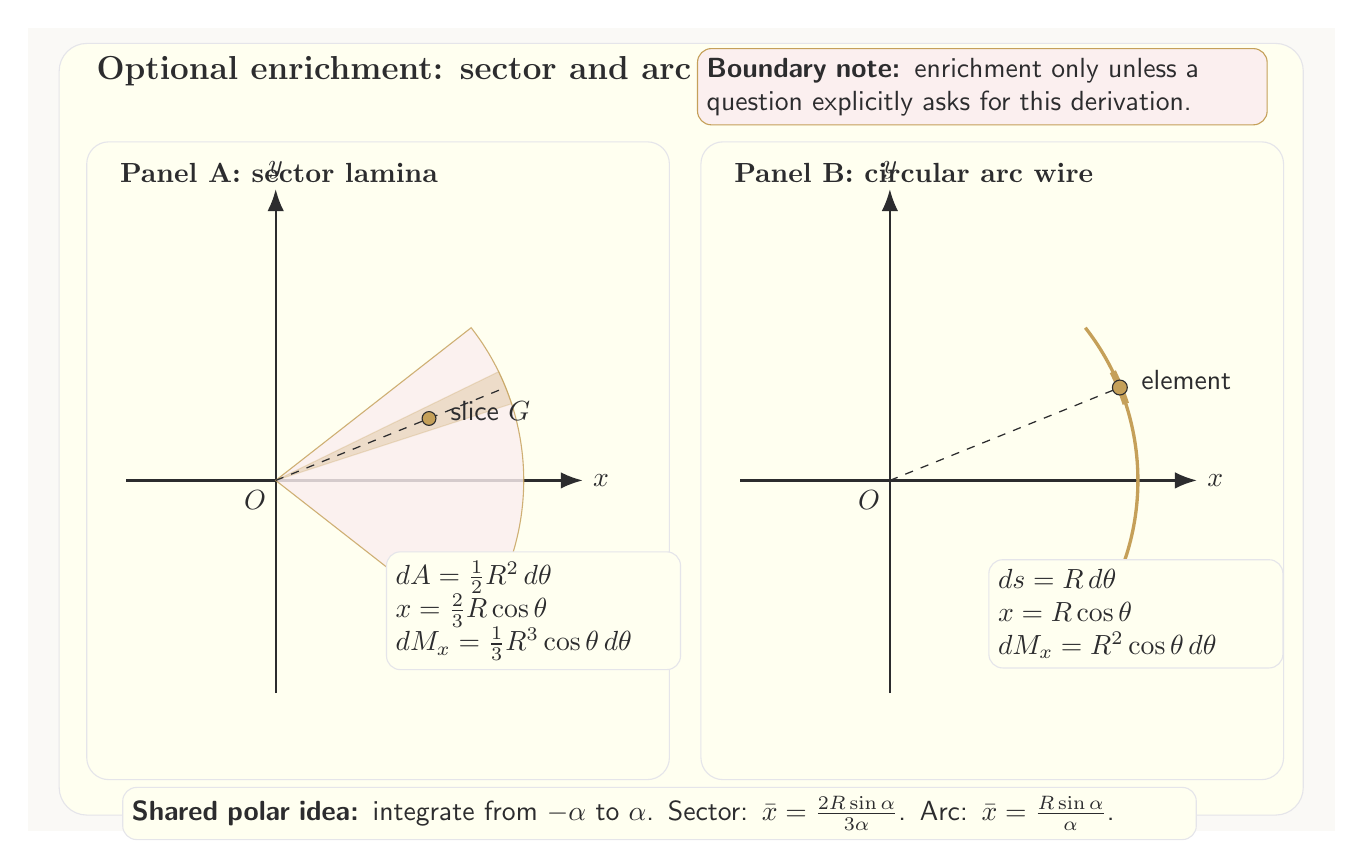
\begin{tikzpicture}[every node/.style={font=\sffamily,text=ink},axis/.style={ink,line width=.8pt,-{Latex[length=2.8mm]}},main/.style={gold,line width=1.2pt},guide/.style={ink,line width=.45pt,dashed}]
\fill[canvas] (-1,-3.2) rectangle (15.6,7);\draw[linegray,fill=ivory,rounded corners=10pt] (-.6,-3) rectangle (15.2,6.8);
\node[anchor=west,font=\bfseries\large] at (-.25,6.45){Optional enrichment: sector and arc using polar slices};
\node[draw=gold,fill=softpink,rounded corners=5pt,text width=7cm,anchor=west] at (7.5,6.25){\textbf{Boundary note:} enrichment only unless a question explicitly asks for this derivation.};
\draw[linegray,fill=ivory,rounded corners=8pt] (-.25,-2.55) rectangle (7.15,5.55);\node[anchor=west,font=\bfseries] at (.05,5.15){Panel A: sector lamina};
\coordinate (O) at (2.15,1.25);\def\R{3.15}\def\a{38}\def\t{18}\def\dt{8}
\draw[axis] (.25,1.25)--(6.05,1.25) node[right]{$x$};\draw[axis] (2.15,-1.45)--(2.15,4.95) node[above]{$y$};\node[below left] at (O){$O$};
\path[fill=softpink,draw=gold,opacity=.82] (O)--++(-\a:\R) arc[start angle=-\a,end angle=\a,radius=\R]--cycle;\path[fill=gold,opacity=.25,draw=gold] (O)--++(\t:\R) arc[start angle=\t,end angle=\t+\dt,radius=\R]--cycle;\draw[guide] (O)--++({\t+\dt/2}:\R);
\coordinate (Gs) at ($(O)+({\t+\dt/2}:2.1)$);\fill[gold,draw=ink] (Gs) circle (2.5pt);\node[anchor=west] at ($(Gs)+(.15,.1)$){slice $G$};\node[draw=linegray,fill=ivory,rounded corners=5pt,text width=3.5cm,anchor=north west] at (3.55,.35){$dA=\frac12R^2\,d\theta$\\$x=\frac23R\cos\theta$\\$dM_x=\frac13R^3\cos\theta\,d\theta$};
\draw[linegray,fill=ivory,rounded corners=8pt] (7.55,-2.55) rectangle (14.95,5.55);\node[anchor=west,font=\bfseries] at (7.85,5.15){Panel B: circular arc wire};
\coordinate (Oa) at (9.95,1.25);\draw[axis] (8.05,1.25)--(13.85,1.25) node[right]{$x$};\draw[axis] (9.95,-1.45)--(9.95,4.95) node[above]{$y$};\node[below left] at (Oa){$O$};
\draw[main] ($(Oa)+(-\a:\R)$) arc[start angle=-\a,end angle=\a,radius=\R];\draw[gold,line width=2.4pt] ($(Oa)+(\t:\R)$) arc[start angle=\t,end angle=\t+\dt,radius=\R];\draw[guide] (Oa)--++({\t+\dt/2}:\R);\coordinate (Ga) at ($(Oa)+({\t+\dt/2}:\R)$);\fill[gold,draw=ink] (Ga) circle (2.7pt);\node[anchor=west] at ($(Ga)+(.15,.1)$){element};
\node[draw=linegray,fill=ivory,rounded corners=5pt,text width=3.5cm,anchor=north west] at (11.2,.25){$ds=R\,d\theta$\\$x=R\cos\theta$\\$dM_x=R^2\cos\theta\,d\theta$};
\node[draw=linegray,fill=ivory,rounded corners=5pt,text width=13.4cm,anchor=west] at (.2,-2.98){\textbf{Shared polar idea:} integrate from $-\alpha$ to $\alpha$. Sector: $\bar{x}=\frac{2R\sin\alpha}{3\alpha}$. Arc: $\bar{x}=\frac{R\sin\alpha}{\alpha}$.};
\end{tikzpicture}
\end{document}
